
% Template for Elsevier CRC journal article
% version 1.1 dated 16 March 2010

% This file (c) 2010 Elsevier Ltd.  Modifications may be freely made,
% provided the edited file is saved under a different name

% This file contains modifications for Procedia Computer Science
% but may easily be adapted to other journals

% Changes since version 1.0
% - elsarticle class option changed from 1p to 3p (to better reflect CRC layout)

%-----------------------------------------------------------------------------------

%% This template uses the elsarticle.cls document class and the extension package ecrc.sty
%% For full documentation on usage of elsarticle.cls, consult the documentation "elsdoc.pdf"
%% Further resources available at http://www.elsevier.com/latex

%-----------------------------------------------------------------------------------

%%%%%%%%%%%%%%%%%%%%%%%%%%%%%%%%%%%%%%%%%%%%%%
%%%%%%%%%%%%%%%%%%%%%%%%%%%%%%%%%%%%%%%%%%%%%%
%%                                          %%
%% Important note on usage                  %%
%% -----------------------                  %%
%% This file must be compiled with PDFLaTeX %%
%% Using standard LaTeX will not work!      %%
%%                                          %%
%%%%%%%%%%%%%%%%%%%%%%%%%%%%%%%%%%%%%%%%%%%%%%
%%%%%%%%%%%%%%%%%%%%%%%%%%%%%%%%%%%%%%%%%%%%%%

%% The '3p' and 'times' class options of elsarticle are used for Elsevier CRC
\documentclass[3p,times]{elsarticle}

%% Sout text (bar)
\usepackage{soul}

%% Hyperlinks
\usepackage{hyperref}

%% The `ecrc' package must be called to make the CRC functionality available
\usepackage{ecrc}

%% The ecrc package defines commands needed for running heads and logos.
%% For running heads, you can set the journal name, the volume, the starting page and the authors

%% set the volume if you know. Otherwise `00'
\volume{00}

%% set the starting page if not 1
\firstpage{1}

%% Give the name of the journal
\journalname{Computers \& Geosciences}

%% Give the author list to appear in the running head
%% Example \runauth{C.V. Radhakrishnan et al.}
\runauth{P. R. Larraondo et al.}

%% The choice of journal logo is determined by the \jid and \jnltitlelogo commands.
%% A user-supplied logo with the name <\jid>logo.pdf will be inserted if present.
%% e.g. if \jid{yspmi} the system will look for a file yspmilogo.pdf
%% Otherwise the content of \jnltitlelogo will be set between horizontal lines as a default logo

%% Give the abbreviation of the Journal.
\jid{procs}

%% Give a short journal name for the dummy logo (if needed)
\jnltitlelogo{Computers \& Geosciences}

%% Hereafter the template follows `elsarticle'.
%% For more details see the existing template files elsarticle-template-harv.tex and elsarticle-template-num.tex.

%% Elsevier CRC generally uses a numbered reference style
%% For this, the conventions of elsarticle-template-num.tex should be followed (included below)
%% If using BibTeX, use the style file elsarticle-num.bst

%% End of ecrc-specific commands
%%%%%%%%%%%%%%%%%%%%%%%%%%%%%%%%%%%%%%%%%%%%%%%%%%%%%%%%%%%%%%%%%%%%%%%%%%

%% The amssymb package provides various useful mathematical symbols
\usepackage{amssymb}
%% The amsthm package provides extended theorem environments
%% \usepackage{amsthm}

%% The lineno packages adds line numbers. Start line numbering with
%% \begin{linenumbers}, end it with \end{linenumbers}. Or switch it on
%% for the whole article with \linenumbers after \end{frontmatter}.
%% \usepackage{lineno}

%% natbib.sty is loaded by default. However, natbib options can be
%% provided with \biboptions{...} command. Following options are
%% valid:

%%   round  -  round parentheses are used (default)
%%   square -  square brackets are used   [option]
%%   curly  -  curly braces are used      {option}
%%   angle  -  angle brackets are used    <option>
%%   semicolon  -  multiple citations separated by semi-colon
%%   colon  - same as semicolon, an earlier confusion
%%   comma  -  separated by comma
%%   numbers-  selects numerical citations
%%   super  -  numerical citations as superscripts
%%   sort   -  sorts multiple citations according to order in ref. list
%%   sort&compress   -  like sort, but also compresses numerical citations
%%   compress - compresses without sorting
%%
%% \biboptions{comma,round}

% \biboptions{}

% if you have landscape tables
\usepackage[figuresright]{rotating}

% put your own definitions here:
%   \newcommand{\cZ}{\cal{Z}}
%   \newtheorem{def}{Definition}[section]
%   ...

% add words to TeX's hyphenation exception list
%\hyphenation{author another created financial paper re-commend-ed Post-Script}

% declarations for front matter

\begin{document}

\begin{frontmatter}

%% Title, authors and addresses

%% use the tnoteref command within \title for footnotes;
%% use the tnotetext command for the associated footnote;
%% use the fnref command within \author or \address for footnotes;
%% use the fntext command for the associated footnote;
%% use the corref command within \author for corresponding author footnotes;
%% use the cortext command for the associated footnote;
%% use the ead command for the email address,
%% and the form \ead[url] for the home page:
%%
%% \title{Title\tnoteref{label1}}
%% \tnotetext[label1]{}
%% \author{Name\corref{cor1}\fnref{label2}}
%% \ead{email address}
%% \ead[url]{home page}
%% \fntext[label2]{}
%% \cortext[cor1]{}
%% \address{Address\fnref{label3}}
%% \fntext[label3]{}

\dochead{}
%% Use \dochead if there is an article header, e.g. \dochead{Short communication}

\title{Insights into Precipitation Estimation from Geostationary Satellites using Deep Learning Models.}

%% use optional labels to link authors explicitly to addresses:
%% \author[label1,label2]{<author name>}
%% \address[label1]{<address>}
%% \address[label2]{<address>}

\author[1]{Pablo R. Larraondo}
\author[1]{Luigi J. Renzullo}
\author[1]{Albert I. J. M. van Dijk}

\address[1]{Fenner School of Environment and Society. Australian National University. Canberra, Australia}

\begin{abstract}
%% Text of abstract
\end{abstract}

\begin{keyword}
%% keywords here, in the form: keyword \sep keyword

%% MSC codes here, in the form: \MSC code \sep code
%% or \MSC[2008] code \sep code (2000 is the default)

\end{keyword}

\end{frontmatter}

%%
%% Start line numbering here if you want
%%
% \linenumbers

%% main text
\section{Introduction}
\label{}

Reliable and accurate estimation of surface precipitation over continuous geographical areas remains an active and challenging research topic, with implications for predicting Earth surface processes driven by rainfall, such as water resources generation, flooding and vegetation growth, among others. Models of these processes are very sensitive to precipitation input data and require accurate representations of precipitation in space and time. Different sensors can be used to measure precipitation, with varying levels of accuracy and resolution. Rain gauges remain the most accurate quantitative measurement method for a given location, but the area for which they are representative can be small. Therefore, other sources of information are required to provide adequate spatial detail. Ground-based rainfall radar, satellite radiometers, space-borne radar instruments and numerical weather prediction models constitute nowadays the main sources to estimate precipitation. Each of these sources has its advantages and limitations associated with their inherent reliability, accuracy, coverage and spatiotemporal resolution. Combining or merging different precipitation estimates to generate improved estimations constitutes an important and active area of research in atmospheric science. \citep{gourley2002exploratory,sideris2014real,nerini2015comparative,hasan2016merging}. An important challenge is to identify and incorporate the strengths of each information source through optimal preprocessing, weighting and merging schemes (e.g., \citep{beck2019mswep,beck2020evaluation}). 

Geostationary satellites provide a frequent and reliable source of information describing the state and evolution of the atmosphere over fixed regions of the Earth. Passive geostationary radiometers do not measure precipitation directly; it is indirectly inferred using its relationship with the reflected and emitted signals captured by the sensor. The main advantage of geostationary satellites is their high spatial resolution (0.5-5 km) and frequency (5-15 minutes) compared to other sources.

So far, precipitation retrievals from geostationary satellites have typically been generated using models based on the physics of the atmosphere that relate precipitation to observed radiation in particular spectral bands. Specifically, higher cloud tops from convective cells show colder temperatures in the Infra-Red (IR) channel which are normally related with higher rain rates \citep{scofield1987nesdis,vicente1998operational}. Other bands in the Water Vapour (WV) channels have also been shown to indicate certain types of precipitation. For example, heavy precipitation from deep convective cells can be detected using the difference between IR and WV channels \citep{kurino1997satellite,schmetz1997monitoring}. A disadvantage of these methodologies is the need for comparatively complex methods to tune model parameters for a specific region and precipitation type \citep{aemetsaf2013}. Furthermore, the accuracy of derived precipitation estimates tends to be low specially when evaluated at small scales \citep{arkin1987relationship}.

An alternative approach is to derive a relationship between the observed multi-spectral measurements and the instantaneous precipitation measured using an independent source or methodology. Available methods include machine-learning models that are able to identify and learn the relationship between predictor and precipitation fields. A notable contribution is the PERSIANN-MSA model \citep{behrangi2009persiann}, which has demonstrated the benefit of including other input multi-spectral bands using Artificial Neural Networks (ANNs). More recent studies have built upon the same idea. For example,  \citep{beusch2018satellite} compared the accuracy of generalized linear models and ANNs to estimate precipitation using geostationary satellite data. 

During the last decade, advances in machine learning have spawned a new generation of models based on neural networks that are commonly referred to as Deep Learning \citep{lecun2015deep}. These models have been able to demonstrate a unique capacity to model complex non-linear processes by defining ANNs with a large number of hidden layers. Convolutional Neural Networks (CNNs) are one type of these networks and have been very successful in the field of computer vision. Since their popularisation in the early 2010s, CNNs have achieved unprecedented results in other scientific domains, such as medical imaging \citep{ronneberger2015u} or weather forecasting \citep{larraondo2019data,rasp2020weatherbench}. The advantage of CNN models is their ability to integrate the spatial context that is inherent in image data into the model. Atmospheric processes associated with precipitation usually have well-defined structures. Therefore, the understanding of spatial structure in images beyond the "per-pixel" approach inherent to CNNs could potentially make this type of models very suitable for deriving precipitation from geostationary satellites. 

The application of CNNs for modelling precipitation from geostationary satellites was recently explored in the context of nowcasting \citep{lebedev2019precipitation}. Their findings demonstrate the advantage of using CNNs to incorporate the spatial context by comparing inferior results with those from simpler models trained on individual pixels. Similar CNN models, that introduce temporal dimension, have been explored to enhance precipitation forecasts \citep{sonderby2020metnet}. Unfortunately, neither study provided the models and training data or described them in sufficient detail to be understood or reproduced. However, it appears both studies followed a similar methodological approach, i.e., discretizing the output precipitation estimates into categories, and reducing the problem to a classification task. 
We wished to pursue a different approach by using a similar CNN model to produce quantitative precipitation estimates through a continuous or regression approach. Furthermore, we used publicly available data and published the source code online to ensure reproducibility of the results. Moving beyond the ‘black box’ use of ANNs, we sought to use them to explore the relationship between each spectral band and precipitation, and to identify the combination of bands that provides the most accurate estimates. Specifically, we sought to answer two questions: 
1) Can a CNN and passive geostationary observations be combined to produce precipitation estimates with an accuracy that is commensurate to that of other methods?
2) Which combination of spectral bands produces the most accurate precipitation estimates?



\section{Data and experimental design}

In this section we describe the data sources and post-processing we perform to create a set of datasets used to train and evaluate the accuracy of the proposed deep learning model. The input dataset for our model comes from the Himawari 8 geostationary satellite and the output will come from the IMERG GPM dataset. This section provides a brief introduction to these datasets, the reasons to choose them for performing our experiments and the post-processing performed to be able to train the models.

\subsection{Data}

Himawari 8 is a geostationary satellite operated by the Japan Meteorological Agency \citep{bessho2016introduction}. The satellite is positioned over 140.7$^\circ$ E, and is equipped with a 16-band multi-spectral sensor, the Advanced Himawari Imager (AHI), spanning the wavelength range between [0.4-13.4] \textmu m. The spatial resolution of the generated images varies for the spectral bands and ranges between 0.5 and 2 km and there is a new full-disk image available every 10 minutes.

The spectral bands of Himawari 8 are able to sense the reflected and emitted radiations of the Earth. For this work we focus on the emission bands exclusively as our purpose is to develop a methodology that is independent of time-of-day. Specifically, the spectral region of interest is between 6 - 13 \textmu m, which corresponds to Bands 8 to 16 in Himawari 8. These 9 bands provide consistent information about the Earth's surface and atmosphere conditions during day and night. These are the input data we use to train the models for estimating precipitation.

The Integrated Multi-satellitE Retrievals (IMERG) is an algorithm that combines information from the Global Precipitation Measurement (GPM) satellite constellation \citep{huffman2015integrated}. IMERG provides precipitation estimates for the majority of the Earth's surface with 10-km resolution at 30 minute intervals.

There are three versions of the IMERG product ["Early", "Late", "Final"] which are processed with increasing  latency and accuracy. The "Final" product is a merged satellite-gauge product and becomes available with a latency of around 4 months after observation. IMERG "Final" uses both forward and backward morphing and includes monthly gauge measurements into the algorithm resulting in the most accurate estimations of precipitation from all IMERG products. This is also the version of IMERG used to carry out the experiments in this work.

\subsection{Data preparation}

Himawari 8 and IMERG products are generated using different spatial and temporal resolutions and map projections. In order to be able to train a model that relates emittance data with estimated precipitation, we need to transform the data into a common coordinate reference system and resolution, so grid points represent the same locations on both products. A desirable characteristic for geospatial data in scientific applications is to represent the data using coordinate reference systems that preserve areas. This ensures that the size of a pixel remains invariant independently of its location. This characteristic is specially important when using machine learning methods to derive physical parameters such as precipitation. Non-equal area projections would report different amounts of precipitation depending on the area, misleading the learning process of models. In this work we choose the Australian Albers Equal Area projection (EPSG:3577) as the common projection for both datasets. We use the GDAL library \citep{warmerdam2008geospatial} to reproject the datasets using bilinear interpolation. IMERG is reprojected into 8km pixels whereas Himawari 8 is reprojected using 2km pixels, to match their original resolutions and allow for an even training of the CNN model (this is explained in more detail in the next section).

The IMERG-Final product is generated every 30 minutes aggregating satellite data gathered during half-hour to create an estimate of the precipitation accumulated during each period in [mm/h]. Where as Himawari 8 generates data every 10 minutes. To match the temporal dimensions in both datasets we choose the Himawari 8 image that is closer to the centre of the accumulation period in IMERG. This results in using the [10, 40] minutes timestamps of every hour in Himawari 8 to match the [00-30, 30-60] minutes accumulations of IMERG respectively.

For this study we consider three equal areas in different parts of Australia and a period of 4 months comprising the 1st November 2018 until the 28th February 2019. Each region is a square of 1024 km on the side covering the South-Eastern region (SE), Northern Territory (NT) and Western Australia (WA). Figure \ref{regions} represents the position and extent of these three regions.

\begin{figure}%
    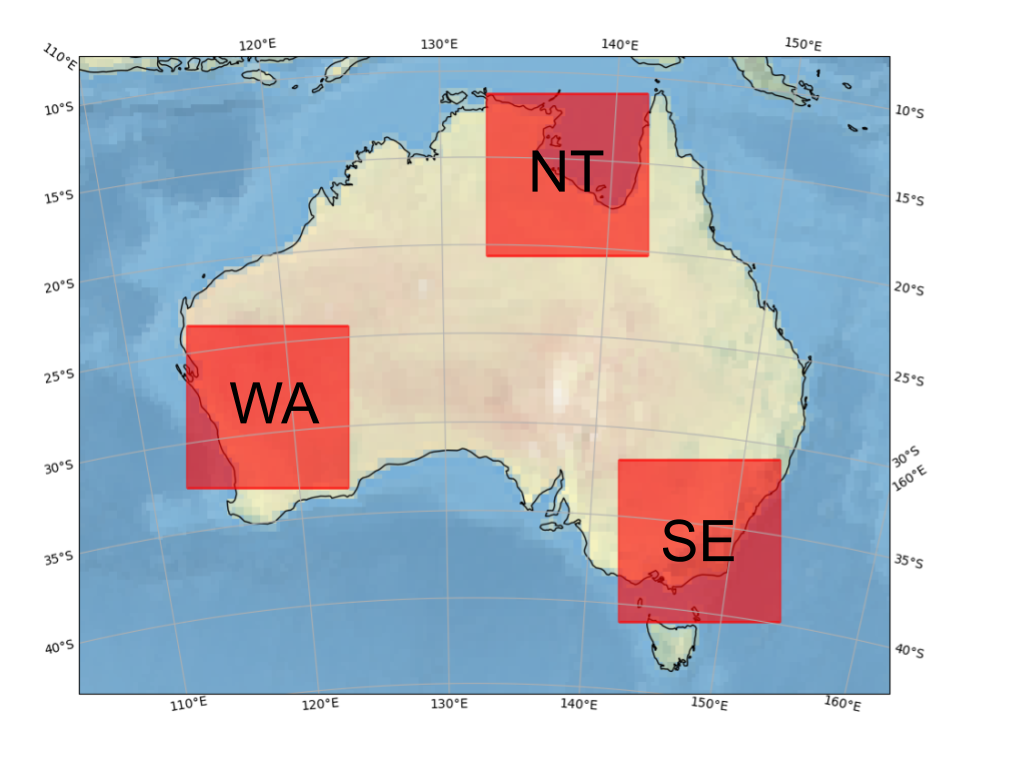
\includegraphics[width=12cm]{regions.png}
    \caption{Geographical location of the three regions used in the experiments.}%
    \label{regions}%
\end{figure}

Each of these regions belongs to different climatic conditions and present different precipitation patterns. The 4 months period comprising November to March covers the majority of the rainy season, when large convective cells develop in the continent. The final Himawari dataset is composed by a set of cubes with 512 points in space along the northing and easting dimensions and 5760 points in time. There are 9 bands and 3 locations which results in 27 cubes of data. In the case of IMERG, after postprossing there are 3 cubes with 128 points in space along the northing and easting dimensions and the same 5760 points in time.

\begin{figure}%
    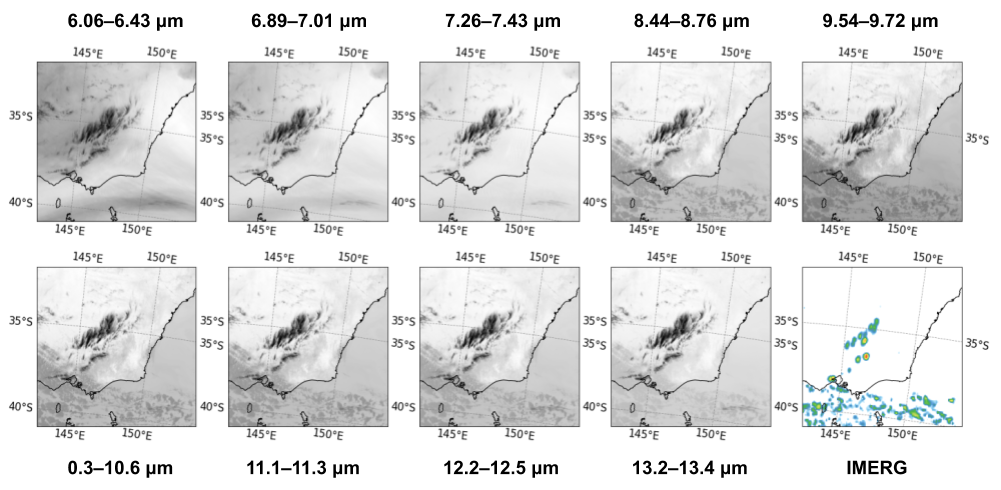
\includegraphics[width=14cm]{dataset.png}
    \caption{Sample of Himawari 8 bands and corresponding GPM precipitations (bottom-right) at for the SE region.}%
    \label{dataset}%
\end{figure}

Figure \ref{dataset} shows one sample in the dataset representing different emission bands from Himawari 8 and the corresponding precipitation retrieved from IMERG product for the SE region. As an example of the different information captured by different parts of the spectrum, we can see how the structure associated with the precipitation in the lower part of Figure \ref{dataset} is only noticeable in the spectral bands above 8 \textmu m. 

\subsection{Model}

To carry out the experiments in this work we use a type of CNN model called U-net \citep{ronneberger2015u}. U-net is an implementation of CNN encoder-decoder which has demonstrated state-of-the-art capacity to learn complex non-linear mappings between image domains generating models that are able to take into account the spatial information and context in the images. Although U-net was originally purposed to segment medical images, later on has found multiple applications in other domains and tasks, such as image regression. In this work we use U-net to learn a model that is able to map between Himawari 8 emission bands and the corresponding precipitation estimation from IMERG. U-net models have been used to estimate precipitation from Numerical Weather Prediction (NWP) gridded geopotential fields \citep{larraondo2019data}. In this work, we use a similar approach applied to higher resolution remotely sensed data to estimate precipitation.

U-nets, and CNN encoder-decoder architectures in general, combine convolution with subsampling (upsampling) operations to compress (decompress) the image space between two domains. In this work we use U-net to learn the relationship between the Himawari 8 emittance domain and the estimated IMERG precipitation. Figure \ref{model_cmp} represents the U-net architecture proposed in this work. Himawari 8 images are the input to the network, on the left of the figure, and IMERG precipitation is the target variable or output, is represented on the right side. The intermediate layers perform convolutions first reducing the spatial extent and expanding the number of channels in the image (encoder) and then the spatial extents in the image are expanded and the number of channels reduced (decoder). As image sizes are halved in each layer of the encoder section, convolution kernels double their spatial domain and are able to find relationships between pixels that are further away. The middle part of the network (bottleneck) contains a compressed latent representation that contains a high-level relationship between the input and output images. The direct (skip) connections between images with same resolutions on the encoder and decoder allow the network to recover the spatial information that would be otherwise lost.

\begin{figure}%
    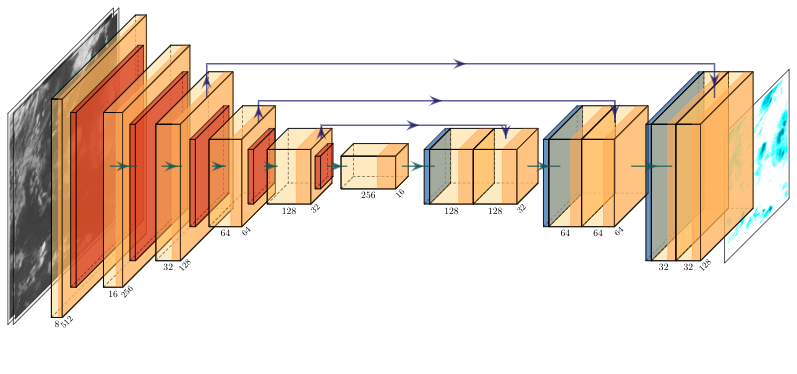
\includegraphics[width=14cm]{unet.png}
    \caption{CNN U-net architecture transforming Himawari 8 input images into IMERG precipitation estimations.}%
    \label{model_cmp}%
\end{figure}

The U-net model used in the experimental section contains a few modifications with respect to the basic implementation. First of all, images from Himawari 8 and IMERG, resulting from the pre-processing step described in the previous section, have different resolutions and require an asymmetrical version of U-net, as represented in Figure \ref{model_cmp}. Another modification introduced in our U-net model is the application of a Rectified Linear Unit (RELU) operation in the last layer of the network to eliminate negative values in the output of the network. This operation constraints the model to generate only positive values in accordance with reality. Finally, we use a loss function based on the Mean Squared Error (MSE), so the model can learn to estimate precipitation quantitatively. This differs from the original implementation of U-net, was initially designed to perform segmentation, a type of classification task. The model presented in this work is implemented using \citep{chollet2018keras} and the code to reproduce the experiments presented in this manuscript are available at: \href{https://github.com/prl900/unet_him8_gpm}{https://github.com/prl900/unet\_him8\_gpm}.

\subsection{Experimental design}

To evaluate the performance of the proposed model he experiments presented in this section are divided in two parts. First we perform a variable selection process over the Himawari 8 bands. The objective is to identify the bands that are more related to precipitation and their relative importance. The second part builds upon these results and performs a comparison between the accuracy the proposed model with other baseline machine learning and physics based methodologies.

The variable selection process aims at identifying the Himawari 8 bands that generate the most accurate models for estimating GPM precipitation. To do this, we started by training identical models using just one band as input and the corresponding GPM precipitation data as output. This first iteration required to train 27 possible models, one for each Himawari 8 emission band, repeated for each geographic area. To train these networks we performed a 4-fold cross-validation, leaving out one month of data each time for testing and training with the remaining three months. Validating on complete months, as opposed to randomised sets, is particularly important here because of the high correlation between temporally close samples. The models are trained using a variation of stochastic gradient descent, which means that the order of the input data determines the model behaviour. To minimise the influence of particular input configurations in the results, we train five versions of each model using different seeds to randomise the order of the input data. This means that to perform this first experiment we train 540 identical models. This number is the product of 3 geographical locations, 9 input bands, 4 cross-validation experiments and 5 seeds to randomise the input data.

Given the large number of models and the size of the data and models we run these models on the CSIRO Bracewell HPC cluster which offers NVIDIA Tesla P100 GPU accelerators. The total training time of this experiment totals more than 1000 hours on specialised high-performance nodes.

To understand the advantage of using CNN models and relative improvement of incorporating the spatial context into the model, we perform a comparison with one physics based model and baseline machine learning method.

First, we compare the output of the resulting model with Convective Rain Rate (CRR) \citep{aemetsaf2013}. CRR is a product originally developed by the Spanish national weather agency (AEMet) to generate convective precipitation retrievals using Meteosat. This methodology was adapted by the Australian Bureau of Meteorology to work with Himawari 8 image and uses the IR Band 8 and (IR-WV) difference using Bands 8 and 13.

The comparison also includes a regression Random Forest (RF) model \citep{breiman2001random} trained on the same data but using individual pixels. This should provide an indication of the relative importance of the spatial context in CNN models.


\section{Results}

 



\subsection{Himawari 8 band selection}

We use categorical statistics to perform the variable selection process using the 0.2 mm/h precipitation threshold. We use two categorical statistics to measure and compare accuracy: recall (aka sensitivity, hit rate or probability of detection) and precision (aka positive prediction value or success ratio). These two metrics can be combined into the F1 score, which allows to assess the accuracy of the models with one value. Figure \ref{experiment_1a} represents a) the recall scores b) the precision scores and c) summarises the previous two scores, using F1 score for the three regions. 

The results presented in Figure \ref{experiment_1a} combine the individual categorical statistics for each band and location resulting from the cross-validation process for different seed values. The accuracy of each band is evaluated aggregating 20 scores (4 cross-validation performed for of the 5 seeds). The box plots represent the distribution and spread in the statistics for each band and location. %Figure \ref{experiment_1a} represents the scores for three categorical scores evaluated using the 0.2 mm/h threshold for the three considered regions.

\begin{figure}%
    \centering
    \subfloat[Precision scores]{{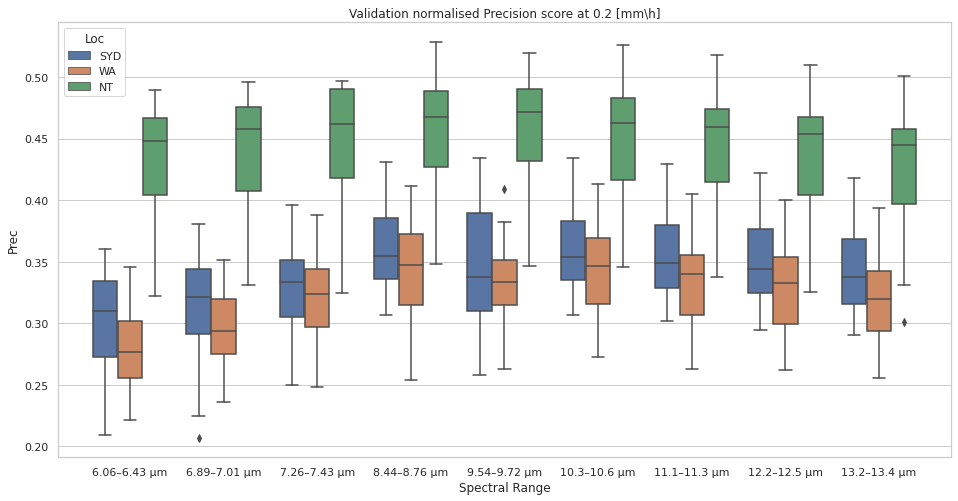
\includegraphics[width=8cm]{figure1a.png} }}%
    \quad
    \subfloat[Recall scores]{{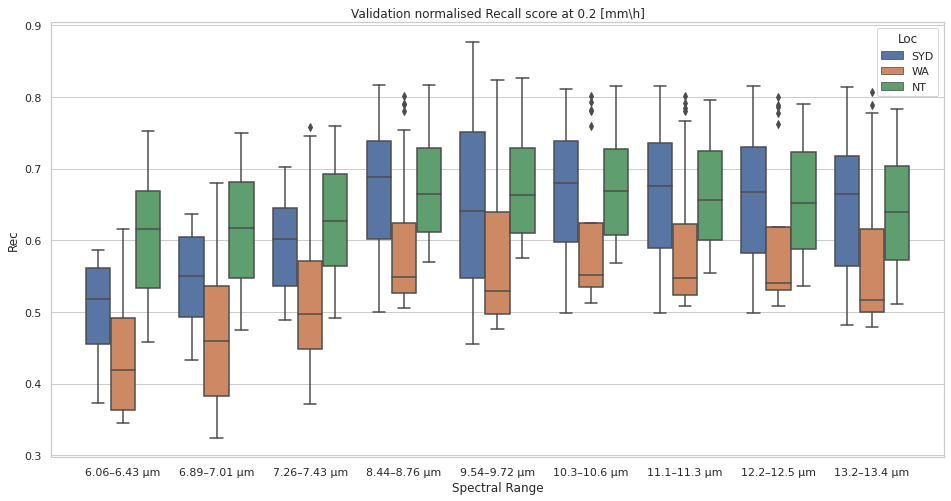
\includegraphics[width=8cm]{figure1b.png} }}%
    % Leave one line blank for new row
    
    \subfloat[F1 scores]{{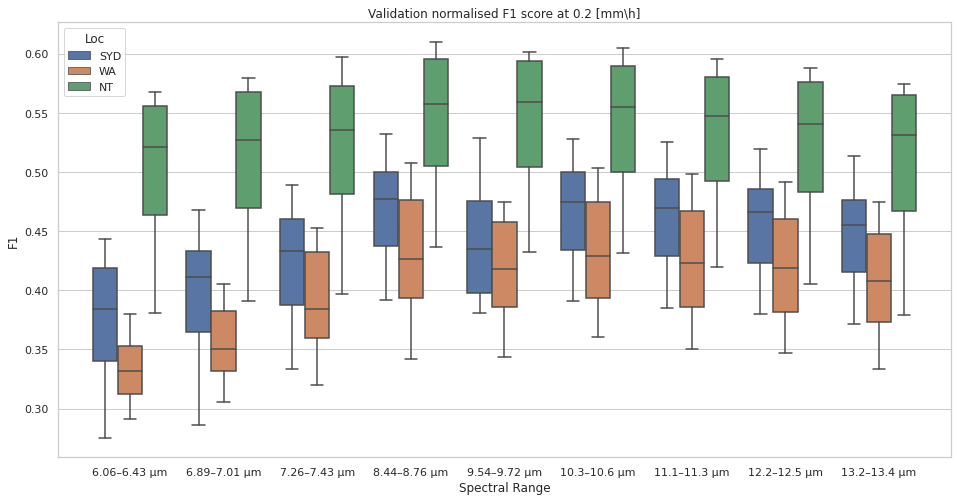
\includegraphics[width=14cm]{figure1c.png} }}%
    \caption{Comparison between (a) precision, (b) recall and (c) F1 scores for the three regions evaluated using a precipitation threshold of 0.2 mm/h}%
    \label{experiment_1a}%
\end{figure}


Figure \ref{experiment_1b} represents the combined F1 scores for a 0.2 mm/h threshold, for the three locations normalised by dividing by the median F1 value of Band 11 [8.44–8.76] \textmu m, which gave the highest score across the three locations. This figure aggregates the results from the three locations and presents a pattern showing higher F1 scores for the bands at the centre of spectrum and a decrease in performance towards the sides. Band 11  m results to be the best performing band in terms of the F1 scores. We acknowledge that the difference in the scores of Bands 11 and 13 might not be statistical significant, however, we choose Band 11 leaving Band 13 as a candidate to be selected in the next iteration of the variable selection process. 

\begin{figure}%
    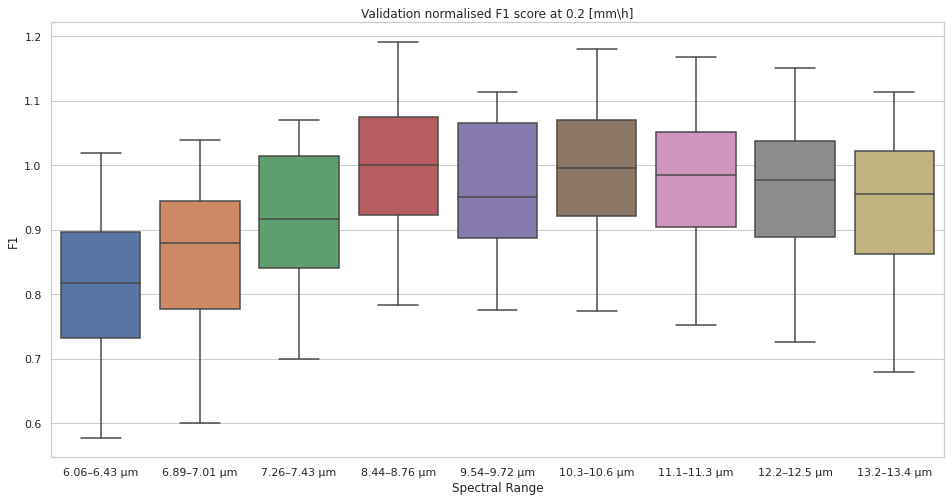
\includegraphics[width=14cm]{figure2.png}
    \caption{Comparison between the combined and normalised F1 scores [0.2 mm/h] for the models trained with each Himawari 8 band.}%
    \label{experiment_1b}%
\end{figure}

We continue the experiment performing a similar iteration using two Himawari 8 bands as input to the models. Due to the large number of models required to iterate through all possible combinations of 9 bands in groups of 2, we reduce this number by fixing Band 11, based on our previous results, and adding the rest of the bands one at a time. Similarly to the first example we train another batch of 520 models.

\begin{figure}%
    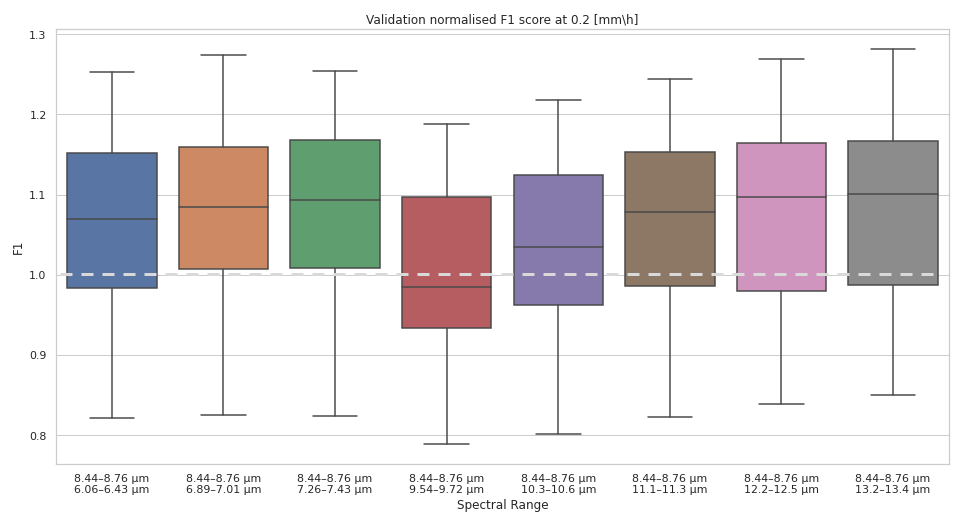
\includegraphics[width=14cm]{figure3.png}
    \caption{Comparison between the combined and normalised F1 scores [0.2 mm/h] for the models resulting from fixing Band 11 and iterating through the rest of the bands.}%
    \label{experiment_2}%
\end{figure}

Figure \ref{experiment_2} represents the validation results for the models trained with two Himawari 8 input bands and normalised using the same median values used in Figure \ref{experiment_1b}. Overall, we observe an increase in the scores compared with the previous figure -- the horizontal gray dotted line represents the best score in the previous step (in this case, Fig. 5). This means that the addition of a new band gives useful information to the model and generates better precipitation estimates. The results in this new figure show a pattern with bands on the sides of the plot performing better than the central ones. This result can be interpreted as the model detecting more valuable information in the bands that are further away in the spectrum to Band 11. For example, Band 8, on the left-hand side, corresponds to wavelengths [6.06–6.43] \textmu m and Band 16, on the right side, corresponds to [13.2–13.4] \textmu m, seem to better complement the information in Band 11 [8.44–8.76] \textmu m than the closer bands. Using this plot we identify the combination of Bands 11 and 16 as the best performing based on their F1 scores.

We perform a new iteration training models with three input bands this time. Following the same process as before, we train a batch of 500 models using Bands 11 and 16, and sequentially add the remaining bands. Figure \ref{experiment_3} represents the F1 scores of the models trained using the different combinations of three input bands -- the horizontal gray dotted line represents the best score in the previous experiment using two bands. F1 scores flatten in this experiment, showing similar and even lower scores compared to the previous experiment. We conclude that adding an extra bands to the combination of Bands 11 and 16 does not improve the accuracy of the considered models. This result suggests that using more than two Himawari 8 bands to train precipitation models does not lead to more accurate estimation. This practice is used in several works in the reviewed literature.

\begin{figure}%
    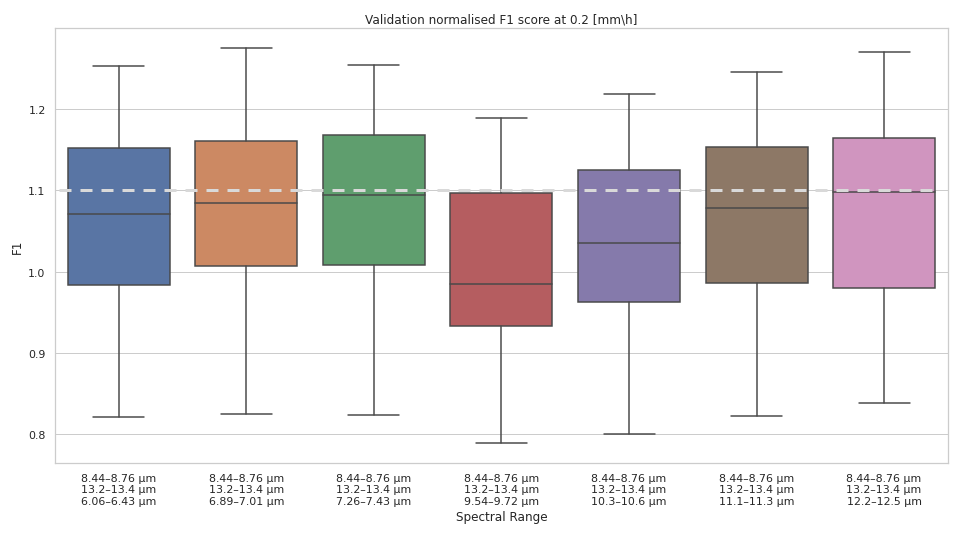
\includegraphics[width=14cm]{figure4.png}
    \caption{Comparison between the combined and normalised F1 scores [0.2 mm/h] for the models resulting from fixing Bands 11 \& 16 and iterating through the rest of the bands.}%
    \label{experiment_3}%
\end{figure}

Figure \ref{output_cmp} offers a visual comparison between the outputs of a selection of these models and the corresponding reference IMERG precipitation. This figure provides a visual understanding of the strengths and shortcomings of the proposed methodology. The visual differences in accuracy between the models are small but we observe an improvement in the precision of the Bands 11 and 16 model compared to the others trained using just one band. In general, the resulting estimated precipitation fields are not able to reproduce the sharp contours and shapes of IMERG. In the presence of clouds, geostationary satellites sense thermal emissions coming mainly from the top part of the clouds. The relationship between emission bands from cloud tops and precipitation seems to be partial and not enough to estimate accurate precipitation considering these results and techniques described.

\begin{figure}%
    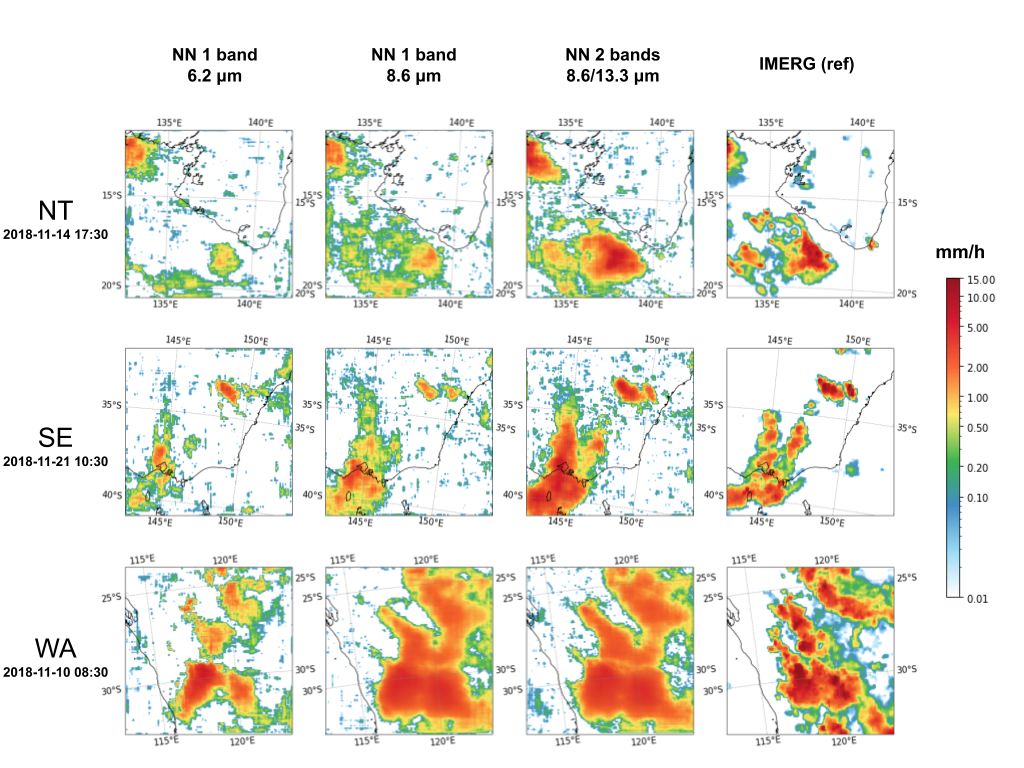
\includegraphics[width=14cm]{output_cmp.png}
	\caption{Visual comparison between the rain estimated by different models trained with Band 8, Band 11, Band 16 and Bands 11 \& 16. The image on the right shows the reference IMERG precipitation}%
    \label{output_cmp}%
\end{figure}

\subsection{Method intercomparison}

To perform this comparison we train the RF and NN models using a similar cross-validation methodology used for the proposed CNN models. Bands 8, 11, 13 and 16 are used as inputs to match the information used by CRR and the CNN models. The precipitation estimations generated by the resulting models and CRR are then compared using the F1 score at different thresholds. These scores are aggregated for the different locations and cross validations. To perform the comparison we use the mean of the ensemble estimations for each pixel.

Figure \ref{model_cmp} offers a visual comparison between the F1 scores obtained for the different models. The CNN model performs significantly better than the other methodologies in the comparison. This is justified by the larger capacity of the model but also its ability to incorporate the spatial context. This is specially noticeable at the higher threshold values, where the superior accuracy of the CNN model is likely to be related to the model's understanding of the size and shape of the associated convective cell.

\begin{figure}%
    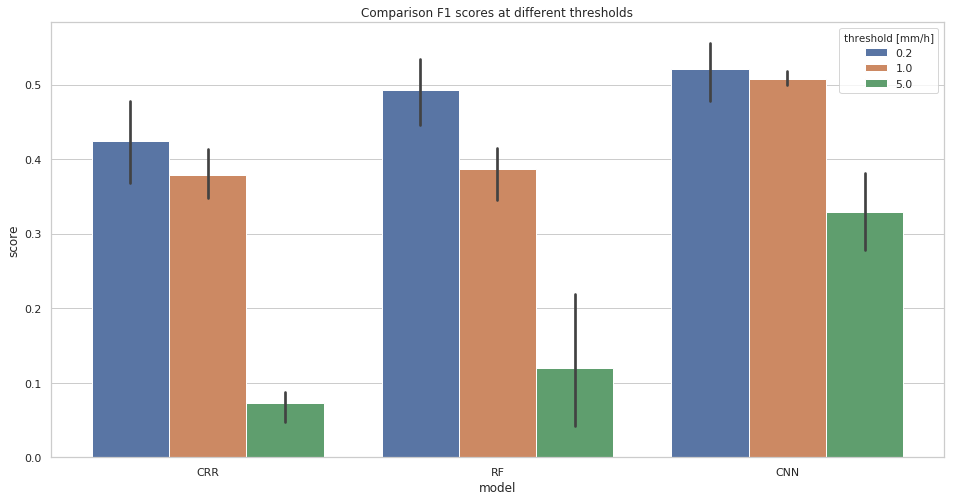
\includegraphics[width=8cm]{model_cmp.png}
    \caption{Comparison between F1 scores between machine learning methods at different rainfall thresholds for the SE region}%
    \label{model_cmp}%
\end{figure}

Figure \ref{baseline_cmp} compares the output of the different models for 3 situations in the validation dataset. We see that although the compared models are able to detect the precipitation areas, the areas with higher intensities are better detected using the proposed U-net model.

\begin{figure}%
    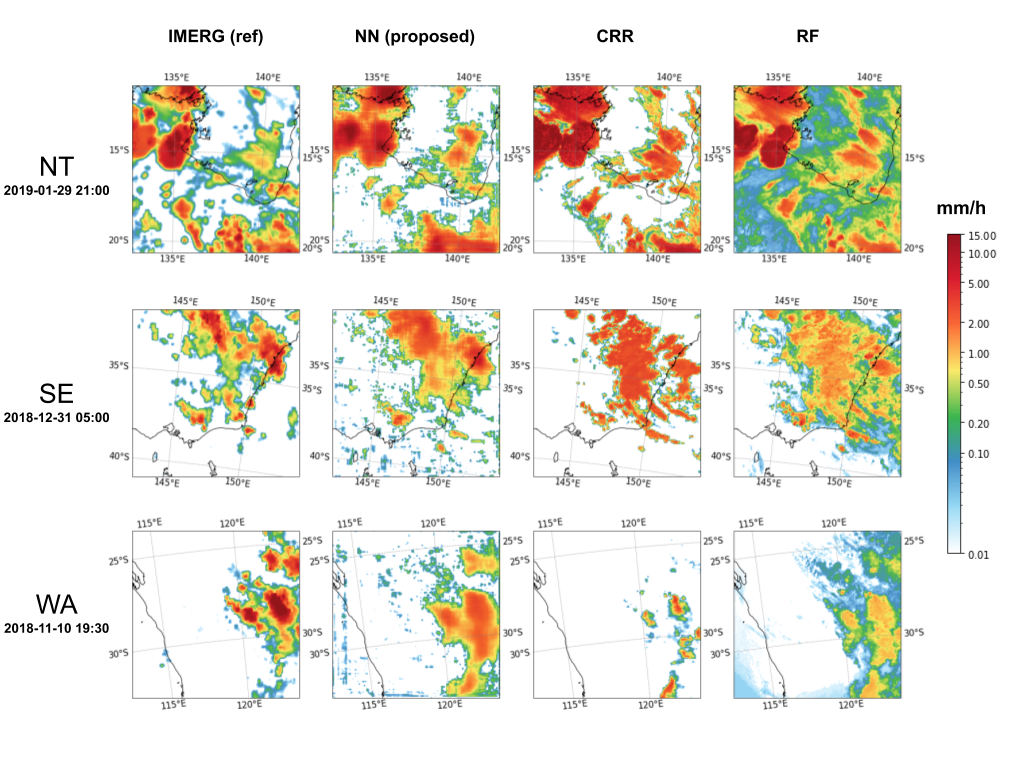
\includegraphics[width=14cm]{baseline_cmp.png}
	\caption{Visual comparison between the output of the different models for different precipitation situations.}%
    \label{baseline_cmp}%
\end{figure}


\section{Discussion}

This work presents the results of an investigation on the application of machine learning methodologies to the problem of estimating precipitation using geostationary satellite images. Remote sensing and precipitation estimation are active and complex research subjects, in which different metrics, datasets and analysis methodologies can be applied. We understand the complexity of the subject and acknowledge the present work only explores a limited and partial area of the whole problem. Nevertheless, we think that the techniques and discoveries hereby presented can be of interest to other researchers and practitioners in this field.

In the presence of clouds, geostationary satellites sense thermal emissions coming mainly from the top part of the clouds. The relationship between emission bands from cloud tops and precipitation seems to be partial and not enough to estimate accurate precipitation considering these results and techniques described.

Another avenue for improving the results presented in this work is to use models that can incorporate the temporal dimension in the data. The atmosphere and precipitation evolves through time following well-defined laws in physics. The high correlation between successive images can provide valuable information to a model for generating estimates that are accurate and consistent through time. There are several approaches that allow incorporating the temporal dimension into neural networks, such as recurrent architectures or 3-dimensional convolutions. The application of these and other architectures and their capacity to incorporate the temporal dimension into the model is something that we also plan to explore. 

Validation of high-resolution precipitation data is highly sensitive to the location and shape of the product. Using measures such as MSE suffer from the double penalty effect penalising estimations that detect the right amounts of precipitation but fail to position in the right location \citep{anthes1983regional,mass2002does}. This is specially relevant when combining data from different sensors and pixels are acquired at different times, as we do in this work. The neural network models considered in the experiments use the MSE loss function which penalise differences on a pixel per pixel basis. Other loss functions based on metrics that account for spatial displacements such as the Wasserstein distance have been proposed in the literature \citep{farchi2016using} and might be better suited for this problem. This a promising area and something we want to explore further in the future.

Given the volume of data and the computational cost of training CNN models, we think that this is a step forward in delivering computationally efficient and accurate precipitation models. In addition, the bands that we identify in this work challenge the traditional practice of using specific IR and WV bands, which opens the door to explore the physical interpretations of the results.

This is what I think should be items for discussion.
\begin{itemize}
    \item Traditionally methods for rainfall estimation from geostationary satellite are based broadly on physical processes and the differential absorption of IR radiation from water vapor and atmospheric window band. This work provides a tool for assessing the relationship and perhaps suggest alternative bands based on available data. 
    
    \item While we focused on geostationary data, we know that there is a fundamental limitation of the approach given uncertainty in cloud-top temperature association with rainfall rate interns if quantity and location. The method we propose can readily incorporate additional independent data, e.g. inputs from NWP like Z (Larraondo et al.)  
    
    \item The difference in performance between study areas (WA, NT, SE) might suggest a need for local model fitting, which can readily[[I guess???]] be done with CNN as opposed to the more traditional calibrated physical modelling approaches.
\end{itemize}

\section{Conclusions}  %% \conclusions[modified heading if necessary]

AvD: "You can start the Conclusions section with a brief recap of the objectives and the experiment, but beyond that focus on summarising and synthesising your main findings and avoid rehashing the methods or results if possible."

This work explores the application of U-net, a deep learning CNN, to estimate precipitation from Himawari 8 retrievals. We propose using IMERG-Final precipitation data to train the models and evaluate the accuracy of the resulting models. To carry out the experiments in this study we consider three locations in Australia, each one defined over squared areas of 1024 x 1024 km and a temporal period spanning four months between the years 2018 and 2019.

The experimental section performs an evaluation to identify the Himawari 8 spectral bands that are able to generate the best precipitation estimations. Band 8, corresponding to wavelengths [6.06–6.43] \textmu m and Band 16 [13.2–13.4] \textmu are identified as the bands that are able to generate models with the most accurate precipitation estimations. The addition of new information, or extra bands, to this type of models does not improve precipitation estimations. \st{The results of the best performing models are then compared with other basic machine learning methodologies and algorithms based on physics for deriving precipitation from geostationary satellites that are used operationally.} The experiments show that the capacity U-nets for incorporating the spatial context presents an improvement when compared to other methodologies applied on individual pixels.

Avd: "A common way to end is to summarise, in one sentence the answer to your hypothesis/es. It often starts with “In summary,..” for example"

%% The Appendices part is started with the command \appendix;
%% appendix sections are then done as normal sections
%% \appendix

%% \section{}
%% \label{}

%% References
%%
%% Following citation commands can be used in the body text:
%% Usage of \cite is as follows:
%%   \cite{key}         ==>>  [#]
%%   \cite[chap. 2]{key} ==>> [#, chap. 2]
%%

%% References with BibTeX database:

\bibliographystyle{elsarticle-num}
\bibliography{references.bib}

%% Authors are advised to use a BibTeX database file for their reference list.
%% The provided style file elsarticle-num.bst formats references in the required Procedia style

%% For references without a BibTeX database:

% \begin{thebibliography}{00}

%% \bibitem must have the following form:
%%   \bibitem{key}...
%%

% \bibitem{}

% \end{thebibliography}

\end{document}

%%
%% End of file `ecrc-template.tex'. 